\subsection{File organization}\label{subsec:file-organization}
%\begin{center}
%    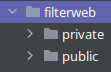
\includegraphics[scale=0.6]{web_main_folder}
%\end{center}
\begin{flushleft}
    In the main folder we can find the next directories:
        \begin{itemize}
            \item public
            \begin{itemize}
                \item In this directory is stored the files available to the user.
            \end{itemize}
            \item private
            \begin{itemize}
                \item In this directory will be stored the files that the user shouldn't have access.
            \end{itemize}
        \end{itemize}
\end{flushleft}

\newpage
\subsection{Public Directory Content}\label{subsec:public-directory-content}

\begin{flushleft}
    Point out that the content of the folder is named .index, to make it more visually appealing, yet this could be
    easily avoided by configuring Nginx, all the php files could follow this structure, it's just a matter of investing
    5 minutes (as much) in doing it.
\end{flushleft}
\begin{center}
    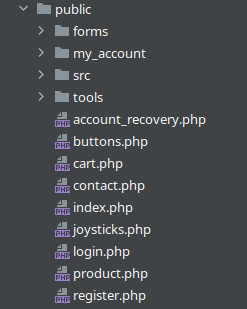
\includegraphics[scale=0.85]{web_public_directory}
\end{center}
In the public folder we can find the next directories:
\begin{itemize}
    \item forms
    \begin{itemize}
        \item Forms used to store the \textbf{API} entry points, used by the client.
    \end{itemize}
    \item my\_account
    \begin{itemize}
        \item Public pages that the user can access in order to manage its account.
    \end{itemize}
    \item tools
    \begin{itemize}
        \item Pages that fulfill a specific function and are often used.
    \end{itemize}
    \item src
    \begin{itemize}
        \item Used to store files that the user might require, mainly used to store:
        \begin{itemize}
            \item Images
            \item JavaScript
            \item Favicon
        \end{itemize}
    \end{itemize}
\end{itemize}
\newpage

\subsection{Private Directory Content}\label{subsec:private-directory-content}
